We can formalize any given \tB{statistical decision problem as a game against nature} (as 
opposed to a game against other strategic players, which is the topic of game theory).
In this game, nature picks a state or parameter $\theta$ or \tB{label, $y\in \mathcal{Y}$, unknown
to us}, and then \tB{generates an observation, $\bm{x}\in\mathcal{X}$} which we get to see. We
then have to make a decision, that is, \tB{we have to choose an action $a$} from some 
\textbf{action space} $\mathcal{A}$. Finally we incur some \textbf{loss}, \tB{$L(y, a)$, which
measures how compatible our action $a$ is with nature's hidden state $y$}.\\
Our goal is \tB{to derive a decision procedure or policy, $\delta: \mathcal{X}\rightarrow
\mathcal{A}$ which specifies the optimal action for each possible input} which specifies the optimal
action for each possible input, meaning the \tR{action that minimizes the expected 
loss}:
$$ \tR{\delta(\bm{x}) = \argmin_{{a\in \mathcal{A}}} \E{{L(y, a)}}} $$
In the Bayesian vision, we mean the expected value of $y$ given the data we have seen so far, 
whereas in the frequentist vision we mean the expected value refers to $x$ and $y$ that we expect
to see in the future.\\
In the Bayesian vision the optimal action having observed $\bm{x}$ is defined as 
\tB{the action $a$ that minimizes the \textbf{posterior expected loss}}:
$$ \tB{\rho(a|\bm{x})\triangleq\mathbb{E}_{p(y|x)}\left(L(y, a)\right) = \su{y}{}L(y,
a) p(y|x)}$$
Hence the \tR{Bayes estimator also called Bayes decision rule is given by:
$$\delta(\bm{x}) = \argmin_{a\in\mathcal{A}}\rho(\bm{a}|\bm{x})$$}
Note that here \uB{we adopted a predictive point of view}, as we took $y$ as reference otherwise it 
would have been a inferential point of view in taking $\theta$.

\subsection{Bayes estimators for common loss functions}
\begin{itemize}
    \item \textbf{MAP} estimate minimizes 0-1 loss: $L(y, a) = \mathbbm{1}_{\{y\neq a\}}
		\begin{cases}
			0 \text{ if } a = y\\
			1 \text{ else}
		\end{cases}$
    \item \textbf{Reject option}, in classification problems where $p(y|\bm{x})$ is very 
		uncertain we may prefer to choose a reject action, in which we refuse to 
		classify the example as any of the specified classes. Let choosing $a=C+1$
		correspond to picking the reject action, and choosing $a\in\{1,...,C\}$
		correspond to picking one of the classes.\\
		$L(y=j, a=i) = 
		\begin{cases}
			0 &\text{ if } i=j \text{ and } i,j\in\{1,...,C\}\\
			\lambda_{r} &\text{ if } i=C+1 \\
			\lambda_{s} &\text{ otherwise}
		\end{cases} $\\
		where $\lambda_{r}$ is the cost of the reject action, and $\lambda_{s}$ is
		the cost of a substitution error. 
    \item \textbf{Squared Error ($l_{2}$)} for a continuous parameters. $L(y, a) =
        (y-a)^{2}$
    \item \textbf{Absolute Error ($l_{1}$)} more robust against outliers. $L(y,a)=
		\lvert y-a\rvert$. The optimal point is the median.
    \item \textbf{Supervised learning} considering a prediction function $\delta: 
        \mathcal{X} \rightarrow \mathcal{Y}$ and some cost function $l(y, \delta(x))$. 
        Then the loss incurred by taking action $\delta$ when the unknown state of nature
        is $\theta$ (the parameters of the data generating the mechanism).
        $L(\bm{\theta}, \delta) \triangleq 
        \mathbb{E}_{(\bm{x}, y)~p(\bm{x},y|\bm{\theta})}\left(
        l(y, \delta(\bm{x}))\right)=\su{\bm{x}}{}\su{y}{}L\left(y,\delta(\bm{x}) 
        p(\bm{x},y|\bm{\theta})\right)$
\end{itemize}

\subsection{Model evaluation metrics}
\begin{itemize}
    \item \textbf{False positive vs False negative trade-off} for binary decision problems
        three are 2 types of errors:
        \begin{enumerate}
            \item {false positive} (false alarm) if $\hat{y}=1 \wedge y=0$
            \item {false negative} (missed detection) if $\hat{y}=0 \wedge y=1$
        \end{enumerate}
        We can consider the loss matrix:\\
        \begin{tabular}{|*{3}{c|}}
            \hline
            \textbf{Headers} & $\bm{y=1}$ & $\bm{y=0}$\\
            \hline
            $\bm{\hat{y}=1}$ & 0 & $L_{FP}$\\
            \hline
            $\bm{\hat{y}=0}$ & $L_{FN}$ & 0\\
            \hline
        \end{tabular}
        where $L_{FN}$ is the cost of a false negative and $L_{FP}$ the cost of a false
        positive.

    \item \textbf{Precision recall curves}
        When trying to detect a rare event the number of negatives is very large, hence
        comparing \emph{sensitivity} and \emph{the error of type I} is not very 
        informative. We would then like to use a measure that only talks about positives.
        \begin{itemize}
            \item \textbf{precision} $=\dfrac{TP}{\hat{N}_{+}}$
            \item \textbf{recall} $=\dfrac{TP}{N_{+}}$
        \end{itemize}
        A \textbf{precision recall curve} is a plot of \textit{precision} vs 
        \textit{recall}.
    \item \textbf{F-scores} is the \emph{harmonic mean of precision and recall}:\\
        $F_{1} \triangleq \dfrac{2}{\frac{1}{precision} + \frac{1}{recall}}$
\end{itemize}


\paragraph{Receiver Operating Characteristic (ROC) curve}
From the below table \\
\begin{tabular}{|cc|*{3}{c|}}
    \hline
    \multicolumn{2}{|c}{\textbf{Headers}} & \multicolumn{2}{|c|}{\textbf{Truth}} &
    \textbf{Count}\\
    \hline
    \multirow{2}{*}{\textbf{Estimate}} & 1 & $TP$ & $FP$ & $\hat{N}_{+}=TP + FP$\\
                                       & 0 & $FN$ & $TN$ & $\hat{N}_{-}=FN + TN$\\
    \hline
    \multicolumn{2}{|c|}{\textbf{Count}} & $N_{+}=TP+FN$ & $N_{-}=FP+TN$ 
                                       & $N=N_{+}+N_{-}=\hat{N}_{+}+\hat{N}_{-}$\\
    \hline
\end{tabular}\\
we can generate the \emph{confusion matrix} is the below table\\
\begin{tabular}{|*{3}{c|}}
    \hline
    \textbf{Headers} & $\bm{y=1}$ & $\bm{y=0}$\\
    \hline
    $\bm{\hat{y}=1}$ & $\dfrac{TP}{N}$ (sensitivity/recall) 
                   & $\dfrac{FP}{N}$ (error type I/ false alarm) \\
    \hline
    $\bm{\hat{y}=0}$ & $\dfrac{FN}{N}$ (error type II/ missed detection) 
                   & $\dfrac{TN}{N}$ (specificity) \\
    \hline
\end{tabular}

Consider \tB{$f(\bm{x})$ a measure of our confidence that $y=1$} like $f=\sigma$, 
however it does not need to be probabilistic simply being monotonically related to 
$\prob{y=1|\bm{x}}$. Let \tB{$\tau$ be  some threshold parameter}, then our 
classification rule is 
$\mathbbm{1}_{\{f(\bm{x})> \tau\}}$. We can then compute TPR(True Positive Rate) also
known as sensibility recall by using \tB{$TPR=\frac{TP}{N_{+}}\approx\prob{\hat{y}=1|
y=1}$}.
As well we are able to compute FPR(False Positive Rate) by using \tB{$FPR=\frac{FP}{
N_{-}} \approx \prob{\hat{y}=1|y=0}$}\\
\tB{ROC is achieved by computing the above TPR and FPR for different value of $\tau$}
Note that 
\begin{itemize}
    \item classifying \uB{everything as negative ($\tau = 1$)} leads to $TPR=0$ and 
        $FPR=0$
    \item classifying \uB{everything as positive ($\tau = 0$)} leads to $TPR=1$ and 
        $FPR=1$
    \item a system working randomly will be close to the diagonal line $TPR=FPR$
\end{itemize}
AUC (Area Under the Curve) summarize the ROC curve


\begin{figure}[H]
    \begin{center}
        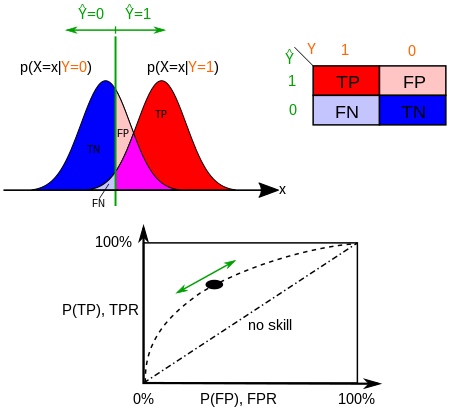
\includegraphics[width=.5\textwidth]{chapters/2_statistics/03_bayesian_approach/images/2_roc_curves_distrib.png}
    \end{center}
    \caption{Receiver Operating Characteristic curve with distribution illustration}
    \label{fig:2_roc_curves_distrib}
\end{figure}
In binary classification the \uB{class prediction for each instance is often made based
on a continuous random variable $X$} , which is the score computed for the instance 
(the estimated probability in logistic regression).\\
X follows a probability density $f_{1}(x)$ if the instance belongs to the class 
"positive" and $f_{0}(x)$ otherwise.\\
Therefore 
$\begin{cases}
    TPR(\tau) = \Su{\tau}{\infty}f_{1}(x)dx \\
    FPR(\tau) = \Su{\tau}{\infty}f_{0}(x)dx
\end{cases}$
and ROC curve plots parametrically $TPR(\tau)$ versus $FPR(\tau)$ with $\tau$ a varying
parameter.\\
Note that this $\tau$ is fundamentally the same that the one above which was squash in
the interval $[0, 1]$


\begin{figure}[H]
    \begin{center}
        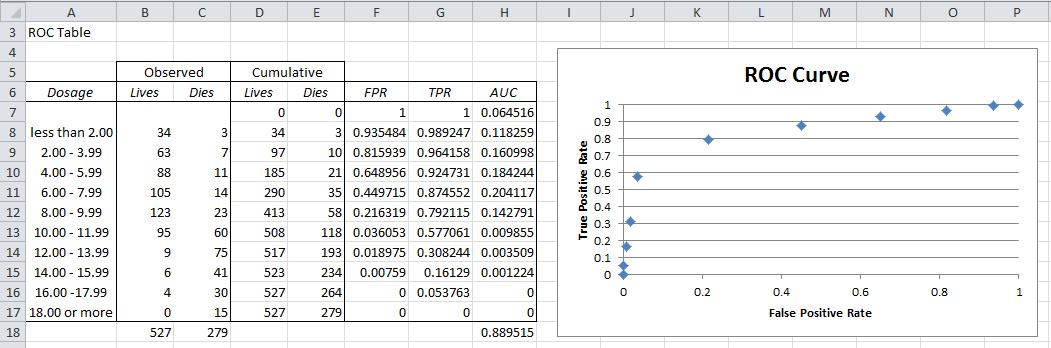
\includegraphics[width=\textwidth]{chapters/2_statistics/03_bayesian_approach/images/1_roc_curve_with_table.png}
    \end{center}
    \caption{Receiver Operating Characteristic curve}
    \label{fig:1_roc_curve_with_table}
\end{figure}
In the above table we have the following formula :
\begin{itemize}
    \item $D9:~SUM(\$B\$7:B9) \rightarrow$ Cumulative Lives
    \item $E9:~SUM(\$C\$7:C9) \rightarrow$ Cumulative Dies
    \item $F9:~1 - D9/\$D\$17 \rightarrow$ False Positive Rate ($1-\frac{TN}{N_{+}}$)
    \item $G9:~1 - E9/\$E\$17 \rightarrow$ True Positive Rate ($1-\frac{FN}{N_{-}}$)
    \item $H9:~(F10-F9)*G9 \rightarrow$ Area Under the Curve
\end{itemize}




